\section{Case Studies}
\label{case-studies}

Our case studies demonstrate the diversity of applications
that can be built on top of the Graffiti API and explore interoperation
between those applications.
The studies also demonstrate some of the unusual design patterns that
Graffiti makes possible when the boundaries between applications
are fuzzy and no one is really in control.

Other than the interoperation we describe, no \emph{unexpected}
interoperation occurs, thanks to our channels concept.
For example, group chat messages do not show up as posts on
a microblogging site even though both use similar object schemas,
because they are each posted to different channels.

All of the applications are written with pure client-side code on
top of the Graffiti Vue plugin.

\subsection{Glitter and The Glue Factory}
%DK Why lump these together?   Describe Glitter first (and discuss how easy it is to implement) than describe Gloof and explain how they interoperate

The following example demonstrates how a community-specific application,
%DK I would call this a social site rather than an application (and explain why).
\emph{The Glue Factory}\footnote{
\url{https://gluefactory.live}\\Source: \url{https://github.com/horseyhouse/glue-factory}
}, can interoperate with a general-purpose application, \emph{Glitter}\footnote{
\url{https://glitter.graffiti.garden}\\Source: \url{https://github.com/graffiti-garden/glitter}
},
without the explicit permission of Glitter.
Not all of the community-specific features on The Glue Factory
translate to Glitter, and not all of the interconnectedness on Glitter
is forced upon The Glue Factory.
Still, there is enough interoperation between the two to be meaningful.

\emph{Glitter} is a text-centric microblogging platform
where users can post, follow, reply, and change their display name.
Replies are threaded and, like Twitter, appear in the replier's followers' feeds, in addition to the reply thread.
There is also a directory that users can add themselves to,
so others can find them.
%DK Is the directory glitter specific?   why?   finding users seems important for most applicatoins.

\emph{The Glue Factory} is an application made for a local
venue to share event flyers.
The flyers are displayed in a grid, similar to Instagram,
but there is just one feed, collectively curated by
the application's fixed set of venue organizers.
Flyers can be replied to, but the organizers may remove replies they disapprove of.

Importantly, The Glue Factory lets
top-level repliers ``crosspost'' their replies
to Glitter, effectively sharing the flyer like a Quote Tweet.
Glitter does not support images and so only the
event description appears.
Replies to the crosspost made on Glitter also appear on The Glue Factory
and vice versa, \emph{unless} The Glue Factory's organizers ``remove'' the reply,
in which case it only appears on Glitter, regardless of where it originated.
Additionally, replies to the crosspost made on Glitter appear in the replier's followers'
feeds while replies made on The Glue Factory only appear in the reply thread,
similar to the difference between Instagram-like and X-like replies described in Section~\ref{concepts:channel-replies}.
Some of this interoperation is shown in Figure~\ref{case-studies:fig:gloof-and-glitter}.

The applications make use of the objects and channels
shown in Figure~\ref{case-studies:fig:schemas-and-channels}.
Importantly, both applications use the same reply object schema,
and the post object schema used by Glitter is a subset of the flyer
object schema used by The Glue Factory.
This overlap makes interoperation \emph{possible},
but selecting ``crosspost to Glitter'' in The Glue Factory intentionally collapses the
channel usage of the two applications,
causing the interoperation to actually \emph{happen}.

\begin{figure*}[t]
    \centering
    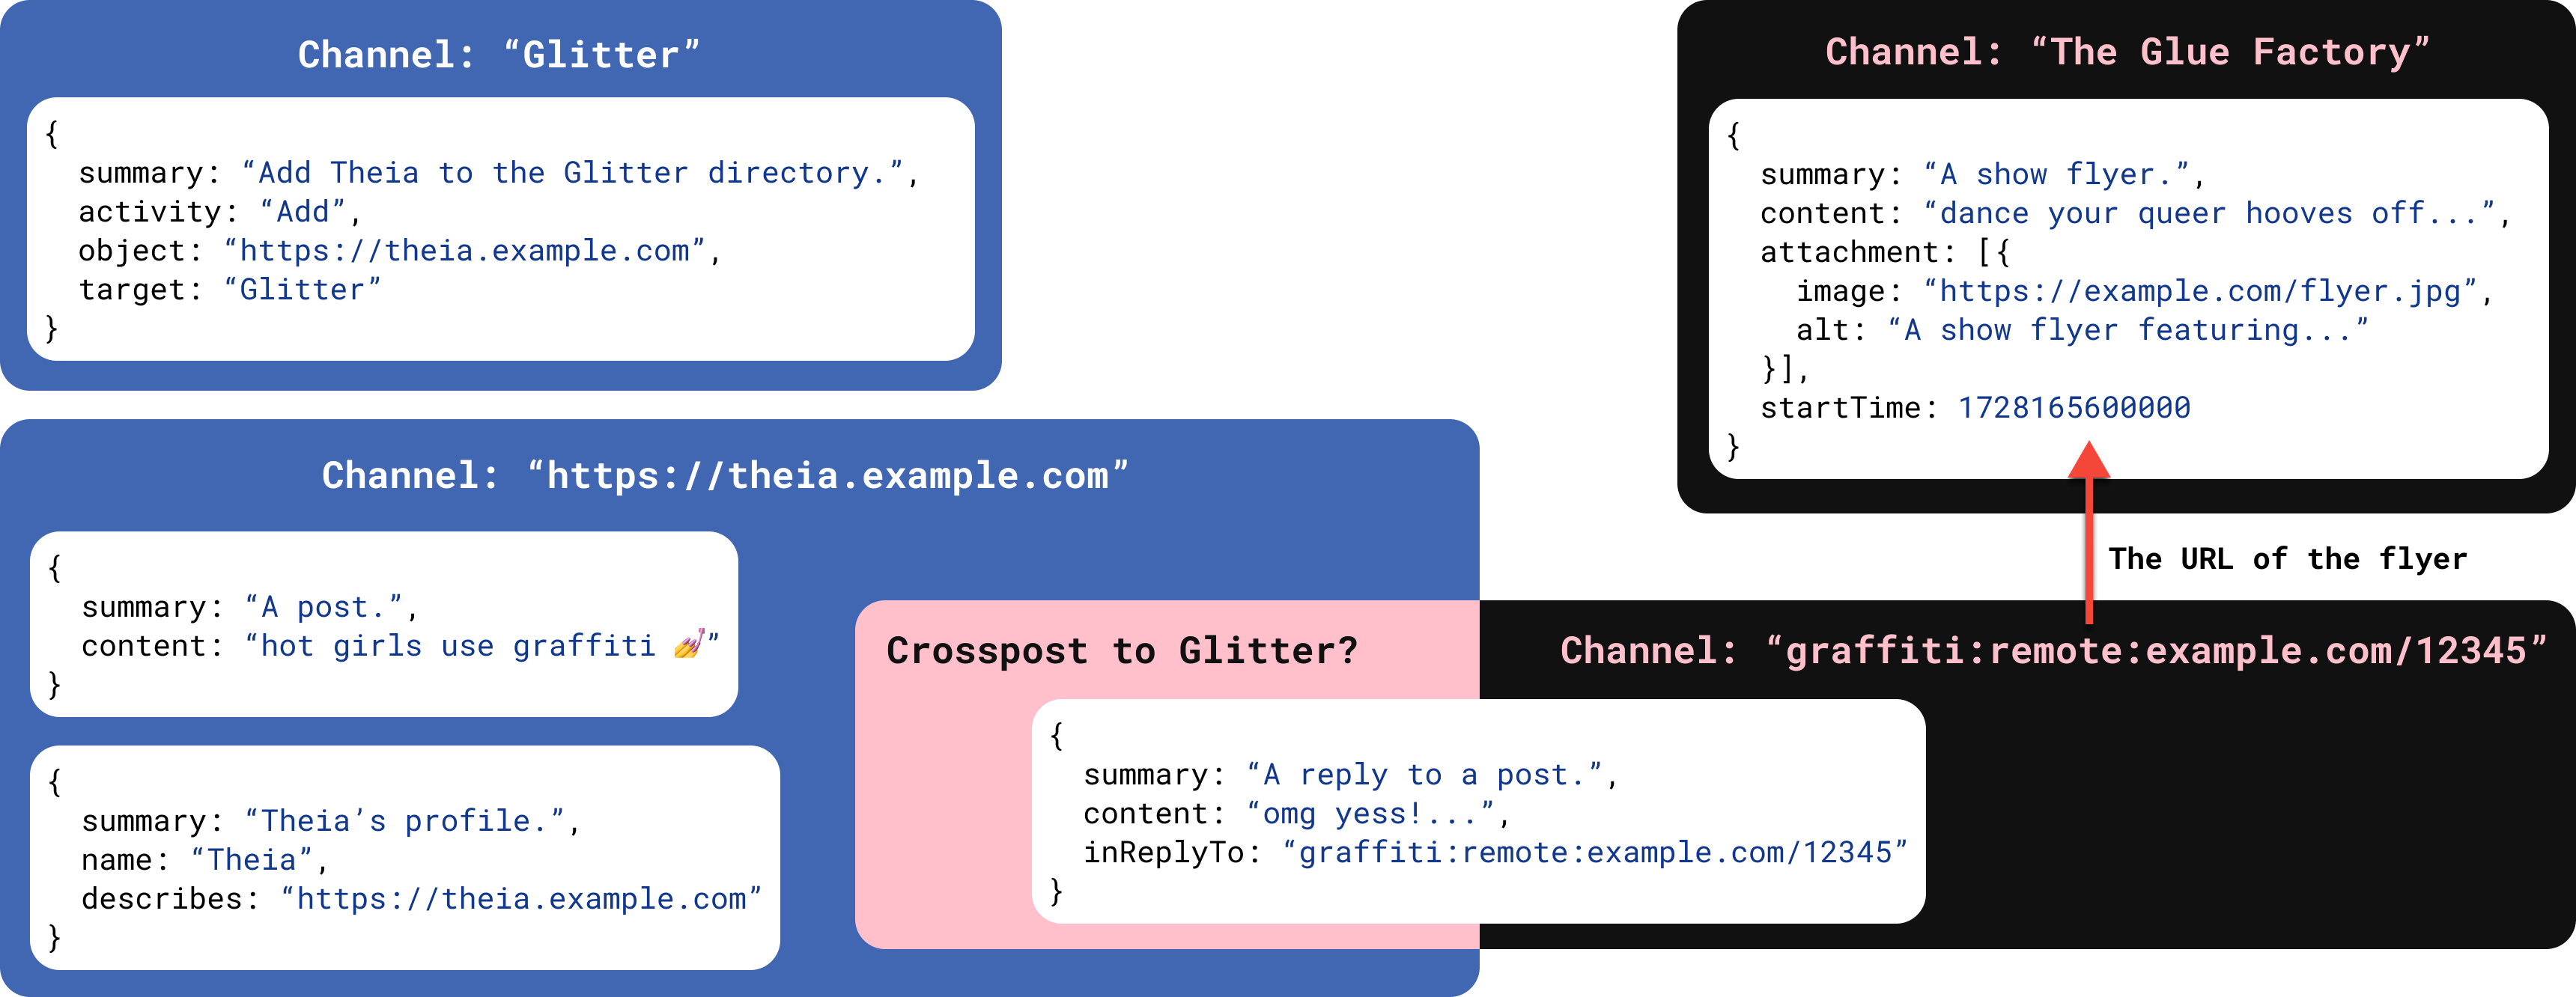
\includegraphics[width=\textwidth]{figures/schemas-and-channels.png}
    \Description{
     The figure shows a series of four rounded rectangles, some overlapping like a Venn diagram, each containing one or multiple JSON blobs. Each rectangle contains at the top a header that says "Channel" followed by a string in quotes and each JSON blob contains a "summary" property. The first rectangle has the channel "Glitter" and contains one JSON blob with the summary "Add Theia to the Glitter directory". The rest of the blob contains { activity: "Add", object: "https://theia.example.com", target: "Glitter" }. The second rectangle has the channel "The Glue Factory" and contains one JSON blob with the summary "A show flyer." The blob also contains { content: "dance your queer hooves off...", attachment: [{ image: "https://example.com/flyer.jpg", alt: "A show flyer featuring..." }], startTime: 1728165600000 }. A third rectangle has the channel "https://theia.example.com" and contains two full JSON blobs and part of one blob that is overlapping with the last rectangle. The first blob has the summary "A post." and one addition property "content" with the value "hot girls use graffiti [nail polish emoji]". The second blob has the summary "Theia's profile." and also contains { name: "Theia", describes: "https://theia.example.com" }. The final blob contains the summary "A reply to a post." and also { content: "omg yess!...", inReplyTo: "graffiti:remote:example.com/12345" }. That blob is contained in a rectangle with the channel "graffiti:remote:example.com/12345". There is an arrow pointing from the channel name of the last rectangle to the blob in show flyer blob in the second rectangle. The arrow is labeled "The URL of the flyer". The overlap between the rectangles with the channels "https://theia.example.com" and "graffiti:remote:example.com/12345" is highlighted and labeled "Crosspost to Glitter?"
    }
    \caption{Example object values and channels used by Glitter and The Glue Factory.
    When crossposting is selected, the reply is put into a Glitter-known channel in addition to a Glue Factory-known one.}
    \label{case-studies:fig:schemas-and-channels}
\end{figure*}

One additional note is that flyers posted to The Glue Factory include a \texttt{startTime}
to display event dates.
This metadata is also used to populate a separate calendar application
used by the co-operative that owns the venue space.

\subsection{Parallax and Provenance}
\label{case-studies:parallax}

%DK perhaps before getting into the crazy bits, talk about how easy it is to implement a basic group chat application ("Grack").   Each group is defined by a channel, and you invite someone to the group by notifyig them about the channel.  There is no admin---anyone in the group can invite others---and no way to remove people without their consent (but you can always create a new group excluding them).  Maybe also describe how you would design a facebook clone ("Gracebook") differently: a user can post content for friends by putting it in their own actorID channel but with an allowlist consisting of their friends.  alternatively they can create a different channel for sharing posts to their friends and invite all friends to subscribe to it.

\emph{Parallax}\footnote{
\url{https://parallax.graffiti.garden}\\Source: \url{https://github.com/graffiti-garden/parallax}
} is a real-time group chat application that demonstrates
how, under total reification, it is possible for \emph{every} user to employ a different
moderation scheme.
Specifically,
every user, from their own perspective,
is the sole administrator of \emph{all} group chats (that they know about) with
unilateral control over each group's name and membership.
The messages a user sends in a group can only be seen by the users they explicitly
put on that group's membership list.
However, users can also see the changes that other users
make to their own ``views'' of a group and are given the option
to \emph{voluntarily} incorporate those changes,
as shown in Figure~\ref{case-studies:fig:parallax}.

\begin{figure*}[t]
    \centering
    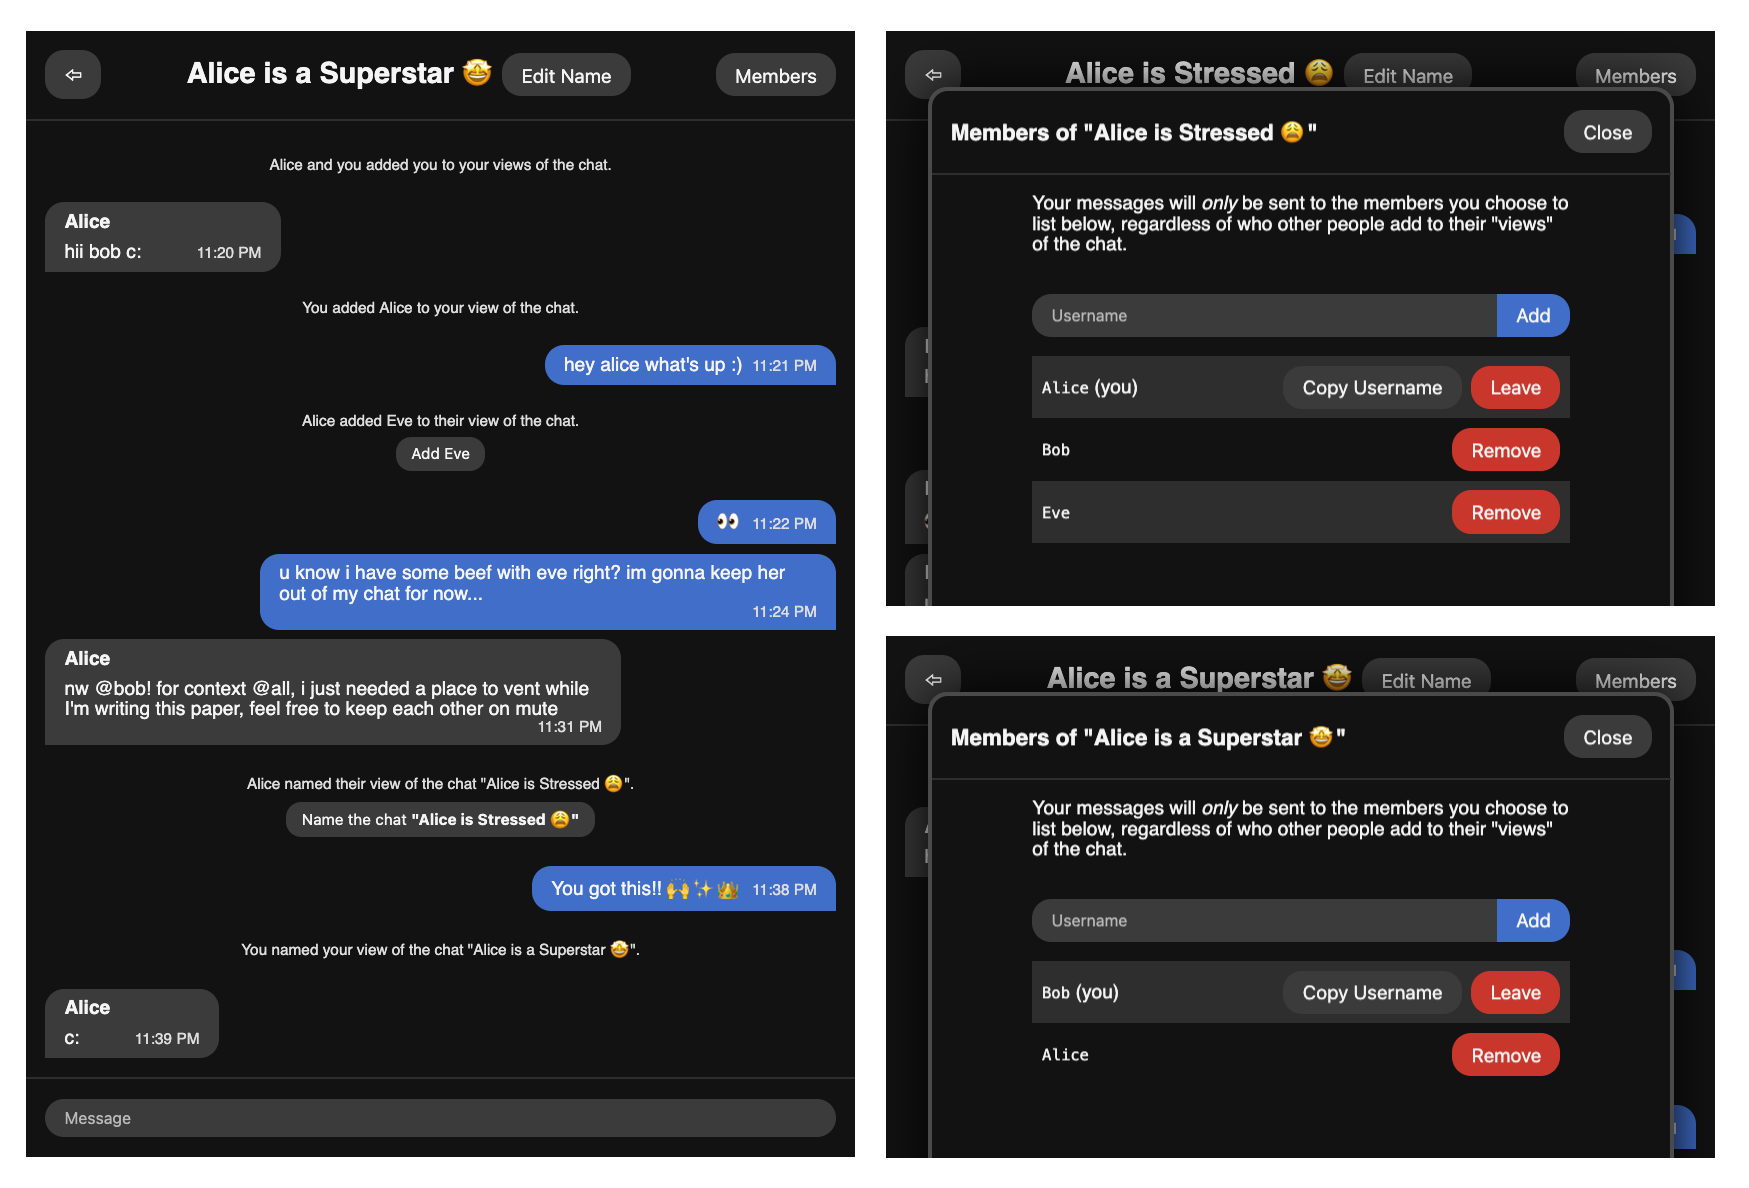
\includegraphics[width=\textwidth]{paper/figures/parallax.png}
    \caption{An interaction on Parallax. On the left is Bob's view of an exchange. On the right are Alice and Bob's \emph{different} membership lists.}
    \Description{
     The figure shows a screenshot of a chat application and cropped screenshots of the "Members" popup in that application. The chat window is titled "Alice is a Superstar [starstruck emoji]" with a button "Edit Name" and a button "Members". Below that the transcript contains both centered text and text in bubbles in either side. Center text: "Alice and you added you to your views of the chat". Left bubble: "Alice: hii bob c:". Center text: "You added Alice to your view of the chat". Right bubble: "hey alice what's up :)". Center text: "Alice added Eve to their view of the chat." and below a button labeled "Add Eve". Right bubble: "[side eye emoji]". Right bubble: "u know i have some beef with eve right? im gonna keep her out of my chat for now...". Left bubble: "Alice: nw @bob! for context @all, i just needed a place to vent while I'm writing this paper, feel free to keep each other on mute". Center text: "Alice named their view of the chat 'Alice is Stressed [weary face emoji]'" and a button "Name the chat 'Alice is Stressed [weary face emoji]'". Right bubble: "You got this!! [raising hands emoji][sparkle emoji][crown emoji]". Center text: "You named your view of the chat 'Alice is a Superstar [starstruck emoji]'". Left bubble: "Alice: c:". Finally there is a message text box. On the right one popup reads "Members of 'Alice is Stressed [weary face emoji]'" with the text "Your messages will *only* be sent to members you choose to list below, regardless of who other people add to their 'views' of the chat." below there is place to enter a username a button "Add" and then finally a list containing "Alice (you)", "Bob", "Eve" with the labels "Leave", "Remove", "Remove" respectively. On the right one popup reads "Members of 'Alice is a Superstar [starstruck emoji]'", containing the same text and form but the members "Bob (you)" and "Alice" with the buttons "Leave" and "Remove" respectively.
    }
    \label{case-studies:fig:parallax}
\end{figure*}

Under the hood, a group is represented by a random identifier,
generated when the group is created, and also used as the group's channel.
A change to a group's name is similar to a profile name change on Glitter, only it
\texttt{describes} the group identifier.
A group's membership can be changed with reified \texttt{"Add"}
and \texttt{"Remove"} activities.
Messages use the same object schema as posts on Glitter,
only they have \texttt{allowed} lists, which are determined
by aggregating the user's own \texttt{"Add"} and \texttt{"Remove"} activities
to determine the group membership state.

Of course, complete independence is not always desirable:
work usually done by just one group administrator must, in Parallax,
be done by every single group user.
We use Parallax to demonstrate an extreme,
but it can be
transformed into a more reasonable (but more restrictive) application called \emph{Provenance}\footnote{
\url{https://provenance.graffiti.garden}\\Source code is in the Parallax repository.
},
where a group's administrator is the \emph{creator} of the group chat.

Parallax and Provenance both interoperate,
but some messages sent from one will not be seen in the other
according to their unequal membership lists. However, this messiness is already present and tolerable
in messaging applications like Signal, where users can block other group members,
and email, where any reply can be sent to a different set of recipients.
There is exciting work to be done learning what interfaces make
Graffiti's inevitable asymmetry most accessible and engaging.

\subsection{Wikiffiti}
\label{case-studies:wikiffiti}

Wikiffiti\footnote{
\url{https://wikiffiti.graffiti.garden}\\Source: \url{https://github.com/graffiti-garden/wikiffiti}
} is a Wikipedia-like application that demonstrates that
collaborative editing in Graffiti is possible,
even though an actor can only mutate their own objects.
Additionally, unlike Wikipedia,
every user on Wikiffiti can choose which other users have ``permission'' to edit an article,
\emph{retroactively} undoing edits by unpermissioned users,
as shown in Figure~\ref{case-studies:fig:wikiffiti}.
The user can only control which users' edits \emph{they} see, not exert any global control---so different users may end up seeing different pages.

\begin{figure*}[t]
    \centering
    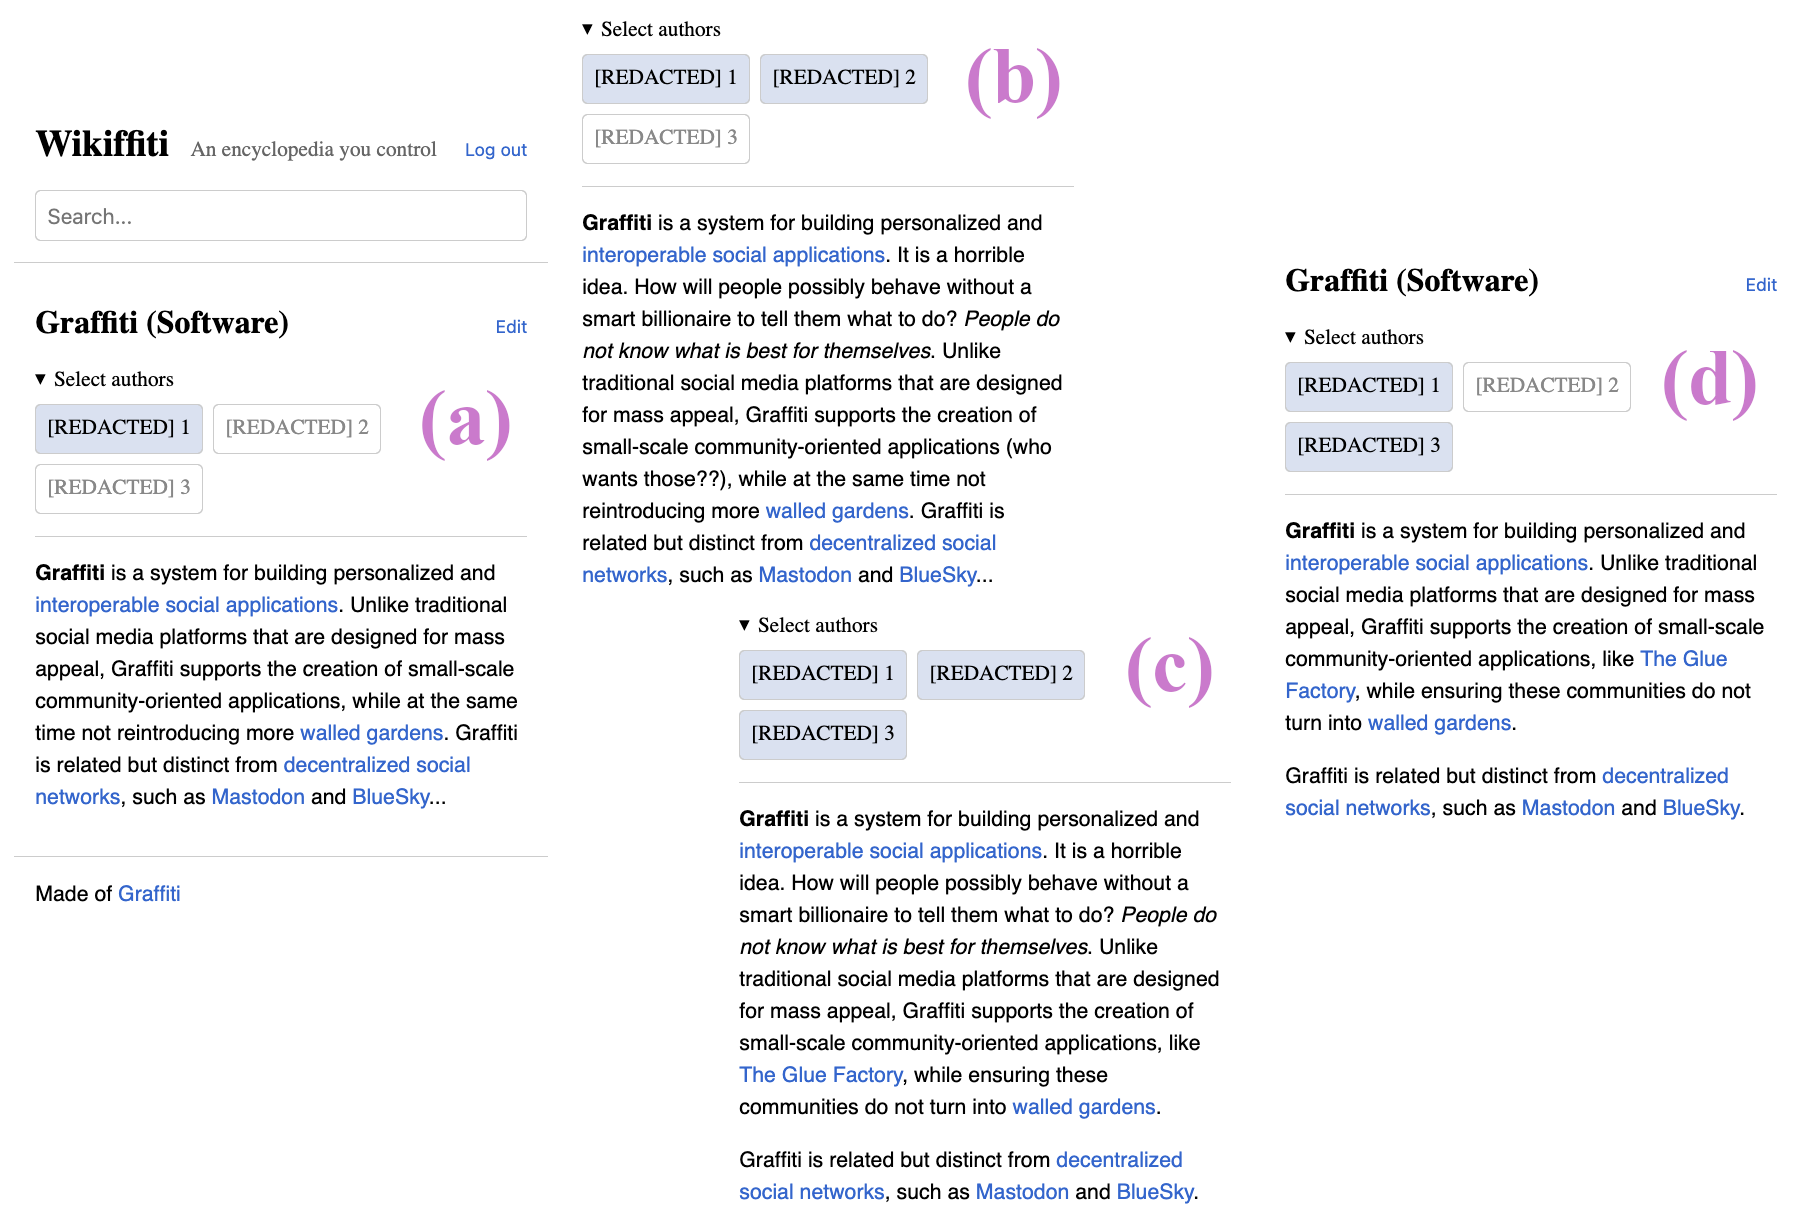
\includegraphics[width=\textwidth]{paper/figures/wikiffiti.png}
    \caption{
    An interaction on Wikiffiti, with changes highlighted for clarity.
    (a) Theia creates a new Wikiffiti page. (b) CEO vandalizes the page. (c) David manually overwrites some of
    CEO's content. (d) All of CEO's edits are retroactively removed.}
    \Description{
    The figure displays four screenshots of a Wikipedia-like application labeled (a) through (d).
    (a) shows the header "Wikiffiti: An encyclopedia you control" with a "Log out" button and a "Search bar". Below, is the title "Graffiti (Software)" a button that says "edit" and an open dropdown listed "select authors" with three buttons labeled "Theia", "CEO" and "David". "Theia" is highlighted, while CEO and David are dimmed. Below, there is the text "Graffiti is a system for building personalized and interoperable social applications. Unlike traditional social media platforms that are designed for mass appeal, Graffiti supports the creation of small-scale community-oriented applications, while at the same time not introducing more walled gardens..
    (b) shows a similar partial interface to that of (a), continuing from the "select authors" on. Now "Theia" and "CEO" are highlighted but "David" is still dimmed. Some of the text is highlighted which we put in brackets. The text reads "Graffiti is a system for building personalized and interoperable social applications. [It is a horrible idea. How will people possibly behave without a smart billionaire to tell them what to do?] Unlike traditional social media platforms that are designed for mass appeal, Graffiti supports the creation of small-scale community-oriented applications [(who wants those??)], while at the same time not introducing more walled gardens.".
    (c) shows the same interface as (a) but now with all buttons selected, "Theia", "CEO", and "David". The text, with bracketed highlights reads "Graffiti is a system for building personalized and interoperable social applications. It is a horrible idea. How will people possibly behave without a smart billionaire to tell them what to do? Unlike traditional social media platforms that are designed for mass appeal, Graffiti supports the creation of small-scale community-oriented applications[, like The Glue Factory], while ensuring these communities do not turn into walled gardens."
    (d) shows the same interface as (a) but now with, "Theia" and "David" selected and "CEO" unselected. The text, with bracketed highlights reads "Graffiti is a system for building personalized and interoperable social applications. Unlike traditional social media platforms that are designed for mass appeal, Graffiti supports the creation of small-scale community-oriented applications[, like The Glue Factory], while at the same time not introducing more walled gardens."
    }
    \label{case-studies:fig:wikiffiti}
\end{figure*}

Edits to each Wikiffiti article are published to
the channel represented by the article's title.
This allows for basic exact-match lookup on titles and, like on Wikipedia,
``disambiguation'' pages can serve as manual search indexes when necessary.

Edits are published and composed together according to Logoot,
a conflict-free replicated data type (CRDT)~\cite{logoot,crdts}.
Logoot, and CRDTs in general, were developed for asynchronous collaborative editing
but, luckily for us, Logoot produces reasonable results when
some edits are ``dropped,'' as we do here intentionally.
Currently, our implementation is inefficient with a 40x space blowup;
however, there are plenty of existing optimizations that one could apply~\cite{logootbetter}
and release as part of a standard collaborative editing library.

Like Parallax, Wikiffiti is an extreme. Clearly not every user
has the expertise or desire to vet all the editors of
every article they read. In reality, the work of approving editors
or individual edits will be delegated to
a hierarchy of user access levels,
friend-of-a-friend networks of trust,
or automatic vandalism detectors, for example.
Still, the data underneath can always be reinterpreted, allowing
for new systems to independently evolve that
might be more welcoming to newcomers~\cite{wikibourgeoisie, wikirisedecline}
or promote edits made by women and non-binary people~\cite{wikigender}.
An application could even highlight edits that are vandalism to some,
but art to others: graffiti.
